\section{Variational Autoencoders~--~VAEs}\label{VAEs}

Generative models play a pivotal role in the field of machine learning, particularly in tasks involving the synthesis and understanding of complex data distributions. Among the diverse types of generative models, Variational Autoencoders (VAEs) stand out for their unique approach and application. These models have gained prominence for their ability to efficiently generate new data samples while capturing the structures of complex data distributions. VAEs operate on the principle of encoding input data into a latent space, a compressed representation of the input data containing only the most important features, and then reconstructing the input from this space. This process is governed by an explicit probabilistic framework, where the model is trained to maximize the likelihood of the data under the learned distribution. This explicit modeling of data distribution in the latent space not only help the generation of new data but also provides valuable insights into the data's inherent characteristics. 

VAEs are essentially based on the architecture of Autoencoders, which apply an iterative process to identify the optimal encoder and decoder pair, aiming to minimize the reconstruction loss while preserving important information after dimensionality reduction. The encoder compresses the input data into a low-dimensional representation, or ``code'' \citep{hintonCode, GoodfellowDeepLearning}, which captures the most relevant features of the input, within a latent space. The decoder's role is to reconstruct the original input from this compressed latent representation. The reconstruction error, which is the discrepancy between the output and the original data, is then used to backpropagate and optimize the model's weights. This process strikes a balance between data compression and information preservation \citep{hintonCode, GoodfellowDeepLearning, michelucci2022introduction}.

Autoencoders, by design, focus on approximate replication of input data rather than perfect replication. This approach necessitates the model prioritizing certain features of the input over others, often leading to the discovery of useful data properties \citep{GoodfellowDeepLearning}. This dimensionality reduction proves beneficial in enhancing classification tasks' efficiency by reducing computational costs and memory overhead, and improving information retrieval in low-dimensional spaces \citep{GoodfellowDeepLearning}. However, traditional autoencoders fall short in generating new data due to the unregulated nature of the latent spaces.

To understand their limitations, consider the analogy of a bag full of numbered balls. If one is tasked with randomly selecting a ball from this bag, the likelihood of picking a specific number is quite low, especially if the bag contains a large number of balls. Each ball in this analogy represents a vector in the latent space of an autoencoder. When an autoencoder extracts features from the input data, the resulting latent space is not perfectly structured; hence, many parts of this space might not correspond to meaningful or recognizable data patterns. This is akin to having many numbers in the bag that do not match the desired number. Thus, when an autoencoder attempts to generate new data by randomly sampling from this unstructured latent space, the likelihood of producing a meaningful output is similarly low. This challenge is further compounded by the fact that the structure of the latent space is influenced by various factors, including the distribution of the source space, the dimensionality of the latent space, and the architecture of the encoder.
\citep{michelucci2022introduction}.

In essence, traditional autoencoders are not designed to generate new data; their main function is to copy and reconstruct the given input \citep{GoodfellowDeepLearning}.

\begin{figure}[ht]
    \centering
      \hspace{.8cm}
      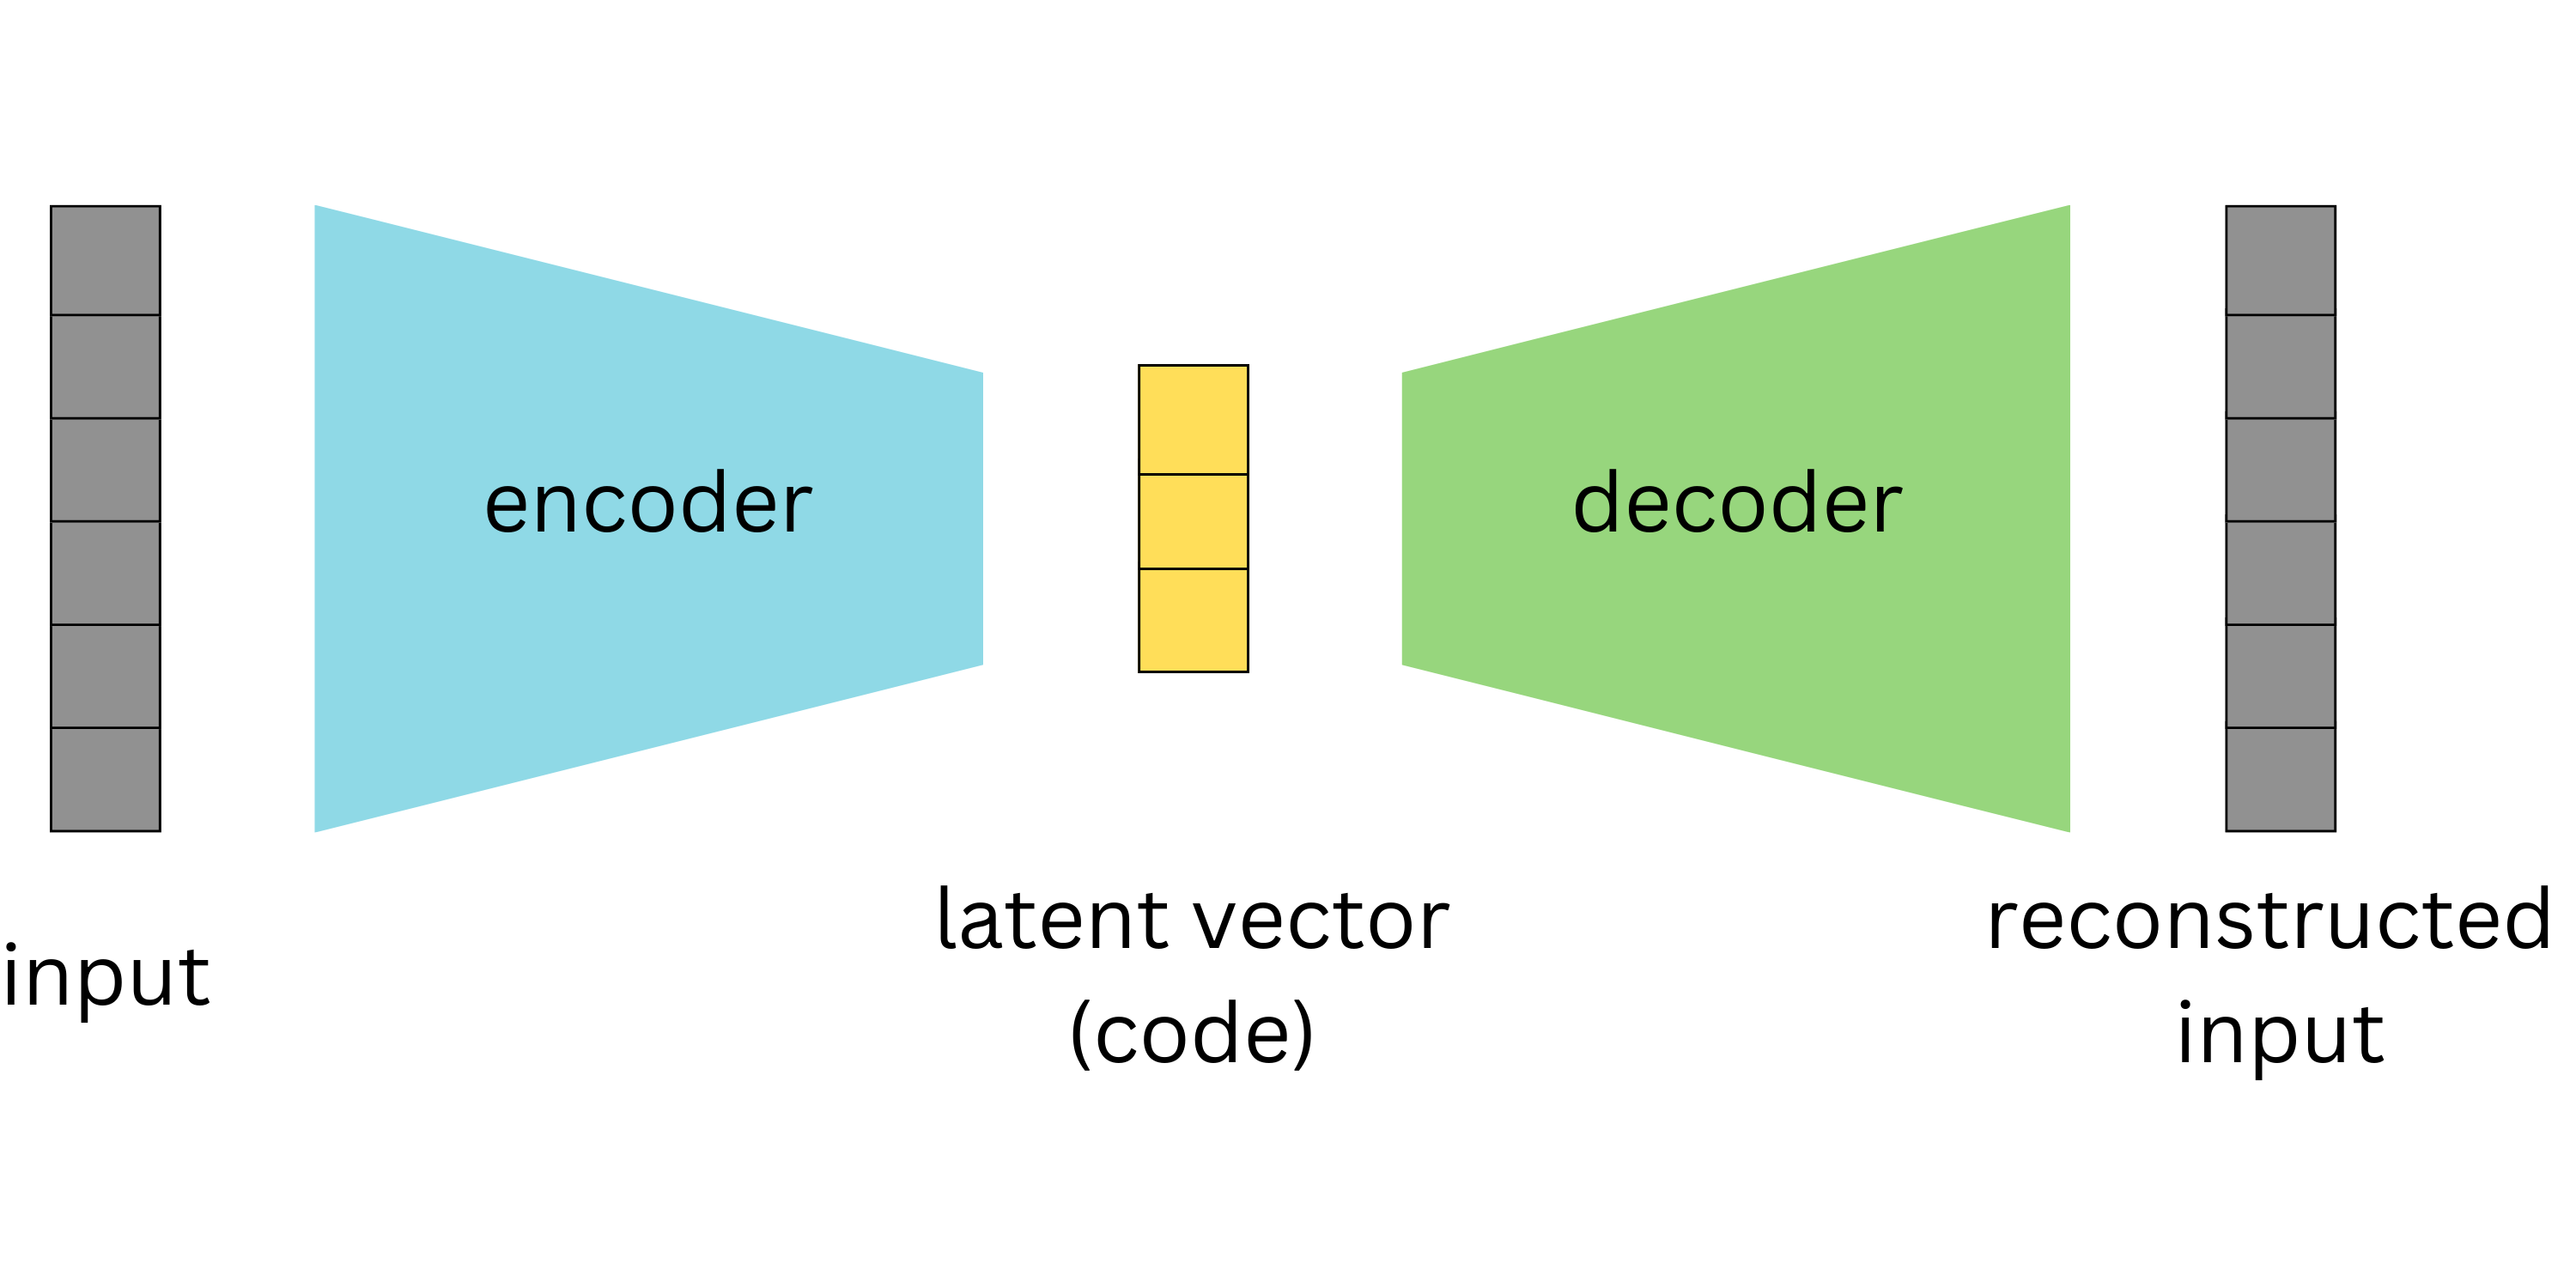
\includegraphics[width=.7\columnwidth]{figures/basics/Autoencoder.png}
      \caption{Schematic of an Autoencoder: Demonstrating the process of dimensionality reduction to a latent vector and subsequent reconstruction, aiming to minimize reconstruction loss.}\label{fig:figureAE}
\end{figure}

At the core of Variational Autoencoders is the handling of the latent space. This approach addresses the limitations of traditional autoencoders by implementing enhanced regularization within the latent space during training. This is achieved by encoding a distribution over the latent space, characterized by parameters \(\mu\) (mean) and \(\sigma\) (standard deviation), instead of encoding to a single deterministic point \citep{doerschVAE}. A key element in this process is the sampling of a point from this distribution to represent the latent variable. This sampled point is then utilized in the reconstruction of the input data, with the resulting reconstruction error being backpropagated to update the model's weights.

To revisit the analogy of the bag full of numbered balls, VAEs transform the scenario. Instead of a bag with a jumble of numbers, VAEs create a more organized bag where regions are filled with specific ranges of numbers. When a ball (a point in the latent space) is selected at random, there's a higher likelihood of it correlating with a meaningful and recognizable pattern, enabling the generation of coherent outputs. This organization within the latent space is key to VAEs' ability to generate new data.

\begin{comment}[
A primary objective of VAEs is the computation of data likelihood, \(P(X)\), through strategic sampling of latent variables \(z\). This aligns with the principle of maximum likelihood, which posits that a model likely to produce samples similar to the training set is preferable. The function \(Q(z|X)\) plays a crucial role here, predicting the most probable latent variables \(z\) that could have generated a given data point \(X\) \citep{doerschVAE}. The core equation of VAEs, as given by \citeauthor{doerschVAE}, encapsulates this relationship:

\[
\log P(X) - D_{KL} \left[ Q(z|X) \parallel P(z|X) \right] = \mathbb{E}_{z \sim Q} \left[ \log P(X|z) \right] - D_{KL} \left[ Q(z|X) \parallel P(z) \right]
\]

This equation first aims to maximize the data's log likelihood (\(\log P(X)\)), indicating the model's effectiveness in accurately recreating data. This term reflects how well the model captures the actual data distribution. Alongside this, the Kullback-Leibler (KL) divergence \(D_{KL}\) serves as a crucial regularization factor. It ensures the model's approximate posterior distribution \(Q(z|X)\) closely aligns with the true posterior distribution \(P(z|X)\), maintaining the integrity of the latent space representation \citep{doerschVAE}. By minimizing this divergence, the model ensures that its encoding of the input data into the latent space is as accurate as possible On the right-hand side, the equation assesses the expected log-likelihood of the reconstructed data from latent variables \(z\), focusing on the model’s decoding accuracy. This ensures that the model can effectively translate the latent space representation back into usable data. Simultaneously, the equation uses another KL divergence term between the posterior \(Q(z|X)\) and the prior distribution \(P(z)\). This divergence helps to regulate \(Q\), ensuring that the latent space corresponds to the prior distribution, which is usually chosen to enable efficient learning and prevent overfitting. 

The optimization of these elements is performed by stochastic gradient descent, where the parameters of \(Q\) are iteratively adjusted to find the optimal balance that allows precise encoding of the input data into the latent space while ensuring a high-quality reconstruction \citep{doerschVAE}
]
\end{comment}


\begin{figure}[ht]
    \centering
      \hspace{.8cm}
      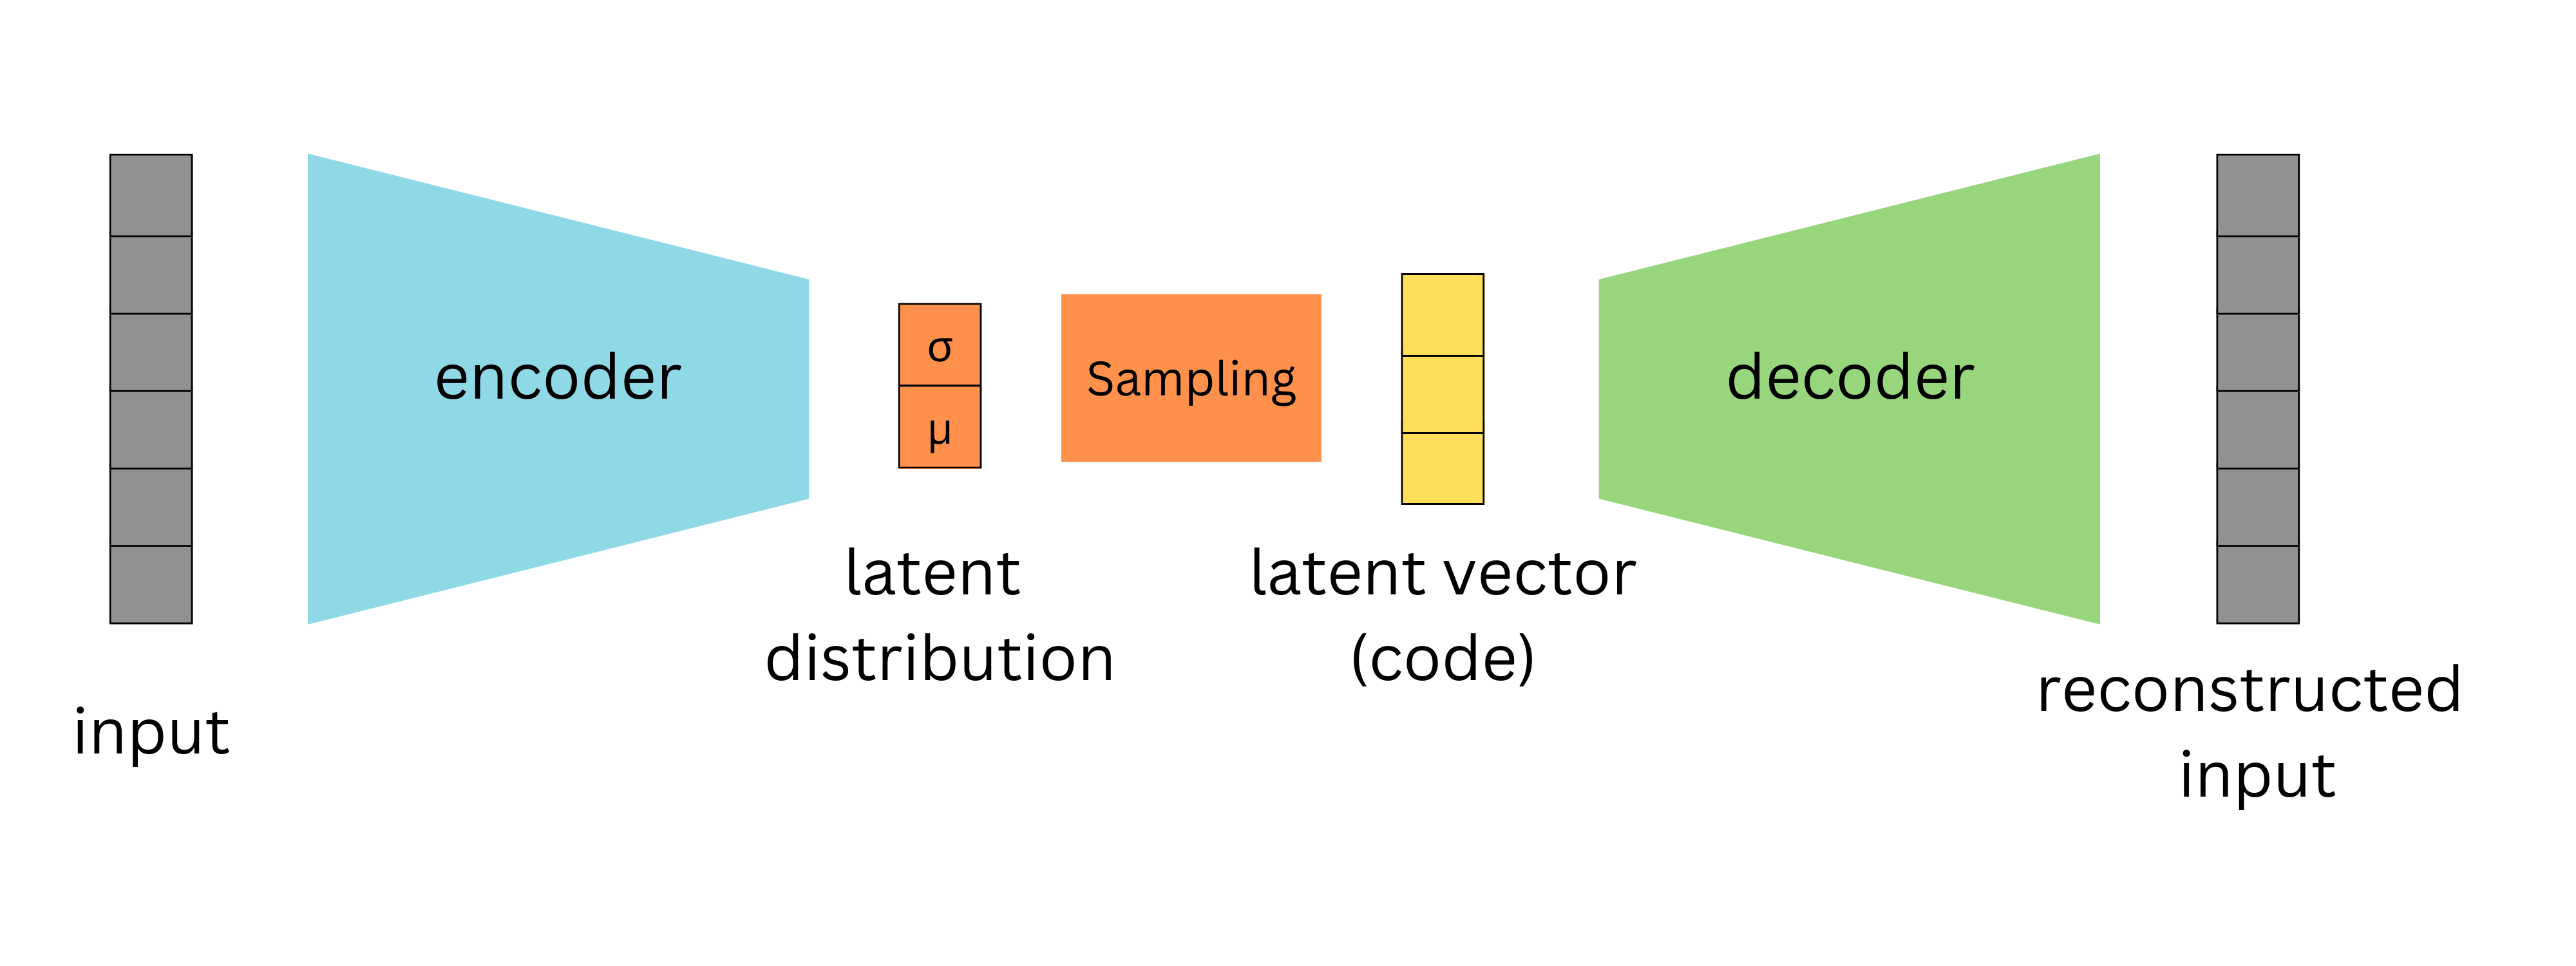
\includegraphics[width=.9\columnwidth]{figures/basics/VAE.png}
      \caption{Functionality of a Variational Autoencoder: This figure illustrates the incorporation of a latent distribution, characterized by mean and standard deviation, for enhancing latent space regularization, enabling more effective and diverse data generation.}\label{fig:figureVAE}
\end{figure}

Despite their advanced capabilities, VAEs have some limitations. A common observation, as noted by \citeauthor{GoodfellowDeepLearning}, is that the generated samples can often appear blurry. This blurriness might stem from the optimization process, specifically the minimization of the Kullback-Leibler divergence. This optimization might lead the model to assign high probabilities to training set points with low `information value' and other less distinct points, resulting in blurry images \citep{GoodfellowDeepLearning}. The Gaussian distribution often used in VAEs for the generative model may also contribute to this effect, as it can ignore minor features in the input data \citep{GoodfellowDeepLearning}. The performance of the model is also sensitive to the choice of priors for the latent space, making hyperparameter tuning an essential aspect of working with VAEs \citep{kingmaVAE, higginsVAE}.
